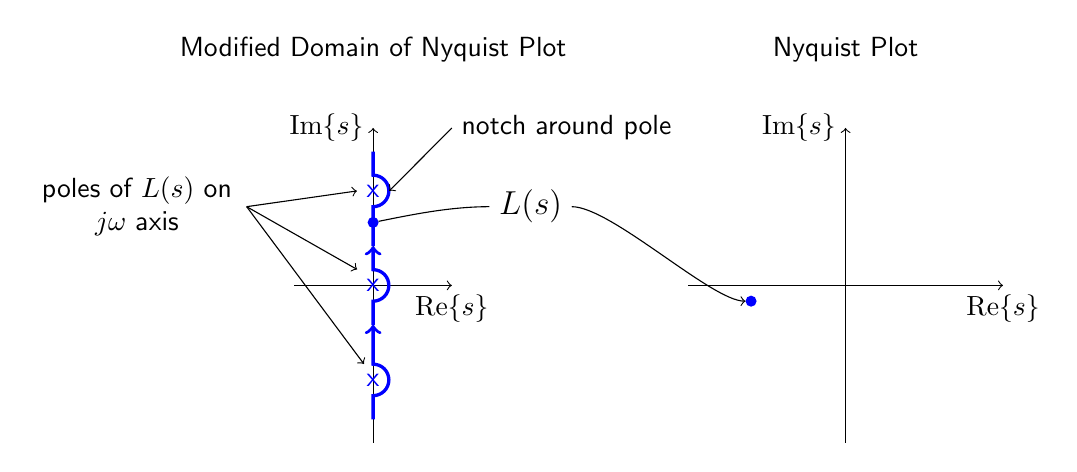
\begin{tikzpicture}[
sysblock/.style={draw,rectangle,inner sep=6pt,minimum width=1.25cm,minimum height=1.0cm,very thick},
summer/.style={circle,draw,very thick}]
\draw (-4,3) node {\textsf{Modified Domain of Nyquist Plot}};
\draw[->] (-4,-2) -- ++(0,4) node[left] {Im$\{s\}$};
\draw[->] (-5,0) -- ++(2,0) node[below] {Re$\{s\}$};
\draw[->,very thick,color=blue] (-4,-1.7) -- (-4,-1.4) arc (-90:90:.2) -- (-4,-.5); 
\draw[->,very thick,color=blue] (-4,-.5) -- (-4,-0.2) arc (-90:90:.2) -- (-4,.5); 
\draw[very thick,color=blue] (-4,.5) -- (-4,1) arc (-90:90:.2) -- (-4,1.7);
%\draw (-4,1.5) node[circle,fill,inner sep=0pt,outer sep=0pt,color=yellow] {\rule{4pt}{0pt}} node[right] {$j\rho$};
%\draw (-4,-1.5) node[circle,fill,inner sep=0pt,outer sep=0pt,color=red] {\rule{4pt}{0pt}} node[right] {$-j\rho$};
%\draw (-4,0) node[circle,fill,inner sep=0pt,outer sep=0pt,color=green] {\rule{4pt}{0pt}};
\draw (-4,.8) node[circle,fill,inner sep=0pt,outer sep=0pt,color=blue] (p1) {\rule{4pt}{0pt}};
\draw (0.8,-0.2) node[circle,fill,inner sep=0pt,outer sep=0pt,color=blue] (p2) {\rule{4pt}{0pt}};
\draw (-4,1.2) node (po1) {\color{blue}\textsf{x}};
\draw (-4,0) node (po2) {\color{blue}\textsf{x}};
\draw (-4,-1.2) node (po3) {\color{blue}\textsf{x}};
\draw (-7,1) node (text) {\begin{minipage}{1in}\begin{center}\textsf{poles of $L(s)$ on $j\omega$ axis}\end{center}\end{minipage}};
\draw (-3,2) node[right] (text2) {\textsf{notch around pole}};
\draw[->] (text.0) -- (po1.180);
\draw[->] (text.0) -- (po2.135);
\draw[->] (text.0) -- (po3.120);
\draw[->] (text2.180) -- (po1.0);
\draw (-2,1) node (L) {\large $L(s)$};
\draw (p1) .. controls ++(.5,.1) and ++(-.5,0) .. (L.180);
\draw[->] (L.0) .. controls ++(.5,0) and ++(-.5,0) .. (p2);

\draw[->] (0,0) -- ++(4,0) node[below] {Re$\{s\}$};
\draw[->] (2,-2) -- ++(0,4) node[left] {Im$\{s\}$};

\draw (2,3) node  {\textsf{Nyquist Plot}};
%\draw[color=blue,very thick] plot[smooth] file {figures/nyquistmapping1.table};
%\draw[color=blue,very thick] plot[smooth] file {figures/nyquistmapping2.table};
%\draw[->,very thick,color=blue] (2,1.485) -- ++(.01,0);
%\draw[->,very thick,color=blue] (2,-1.485) -- ++(-.01,0);

%\draw (2,.026) node[circle,fill,inner sep=0pt,outer sep=0pt,color=yellow] {\rule{4pt}{0pt}} ;
%\draw (2,-.026) node[circle,fill,inner sep=0pt,outer sep=0pt,color=red] {\rule{4pt}{0pt}};
%\draw (3.4,0) node[circle,fill,inner sep=0pt,outer sep=0pt,color=green] {\rule{4pt}{0pt}};

%\draw (-5,-2.5) node[right] {$\rho=$ big enough number so that $L(j \rho)$ approaches a constant};



\end{tikzpicture}